\graphicspath{{chapters/chapter4/img/}}

\chapter{Results and discussion}
\label{cha:results}

This chapter is meant to show and discuss the results obtained from the application of the methods introduced in \Cref{cha:methods}.

\begin{figure}[H]
	\centering
    	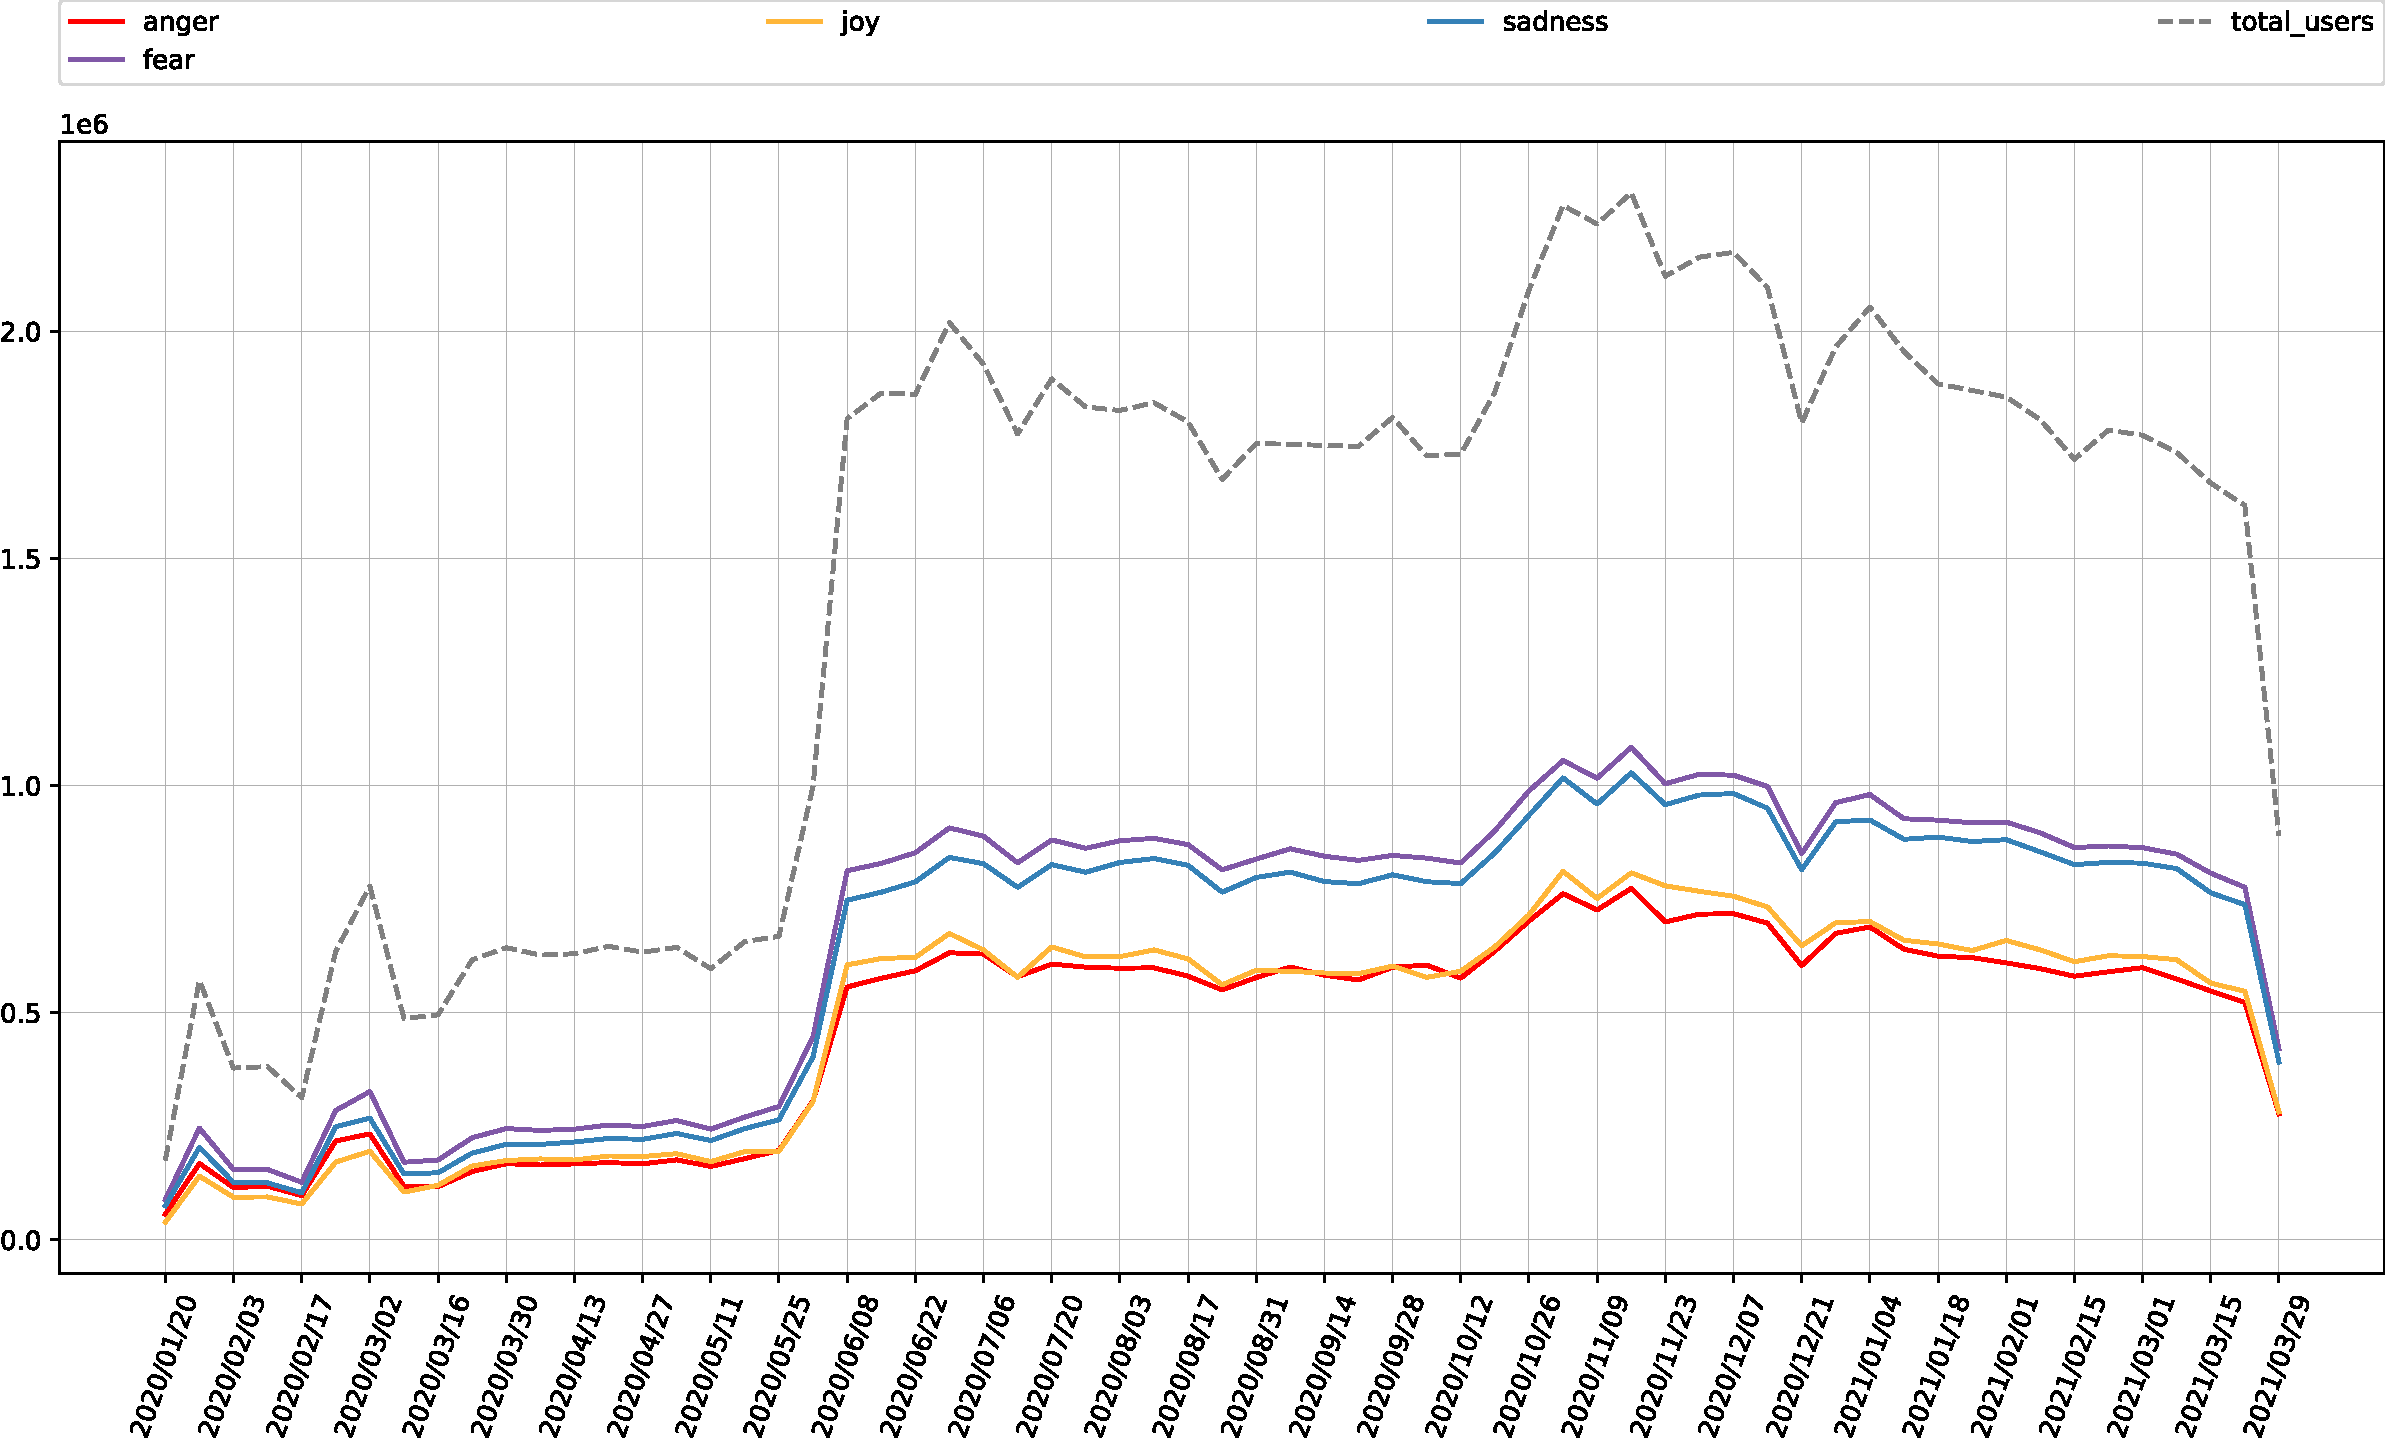
\includegraphics[scale=.35]{en_4_emotions_abs.svg}
    	\caption{Number of weekly users per emotion in the English tweets}
    	\label{fig:en-4-emotions-abs}
\end{figure}

\Cref{fig:en-4-emotions-abs} displays the number of users that expressed a particular emotion in a given week, considering the English tweets. Instead, the gray dashed line indicates the number of users that posted at least one tweet during a week. The fact that the data collection migrated to AWS around June 2020, explains why the number of tweets almost doubled from 2020/06/01 to 2020/06/08.

\begin{figure}[H]
	\centering
    	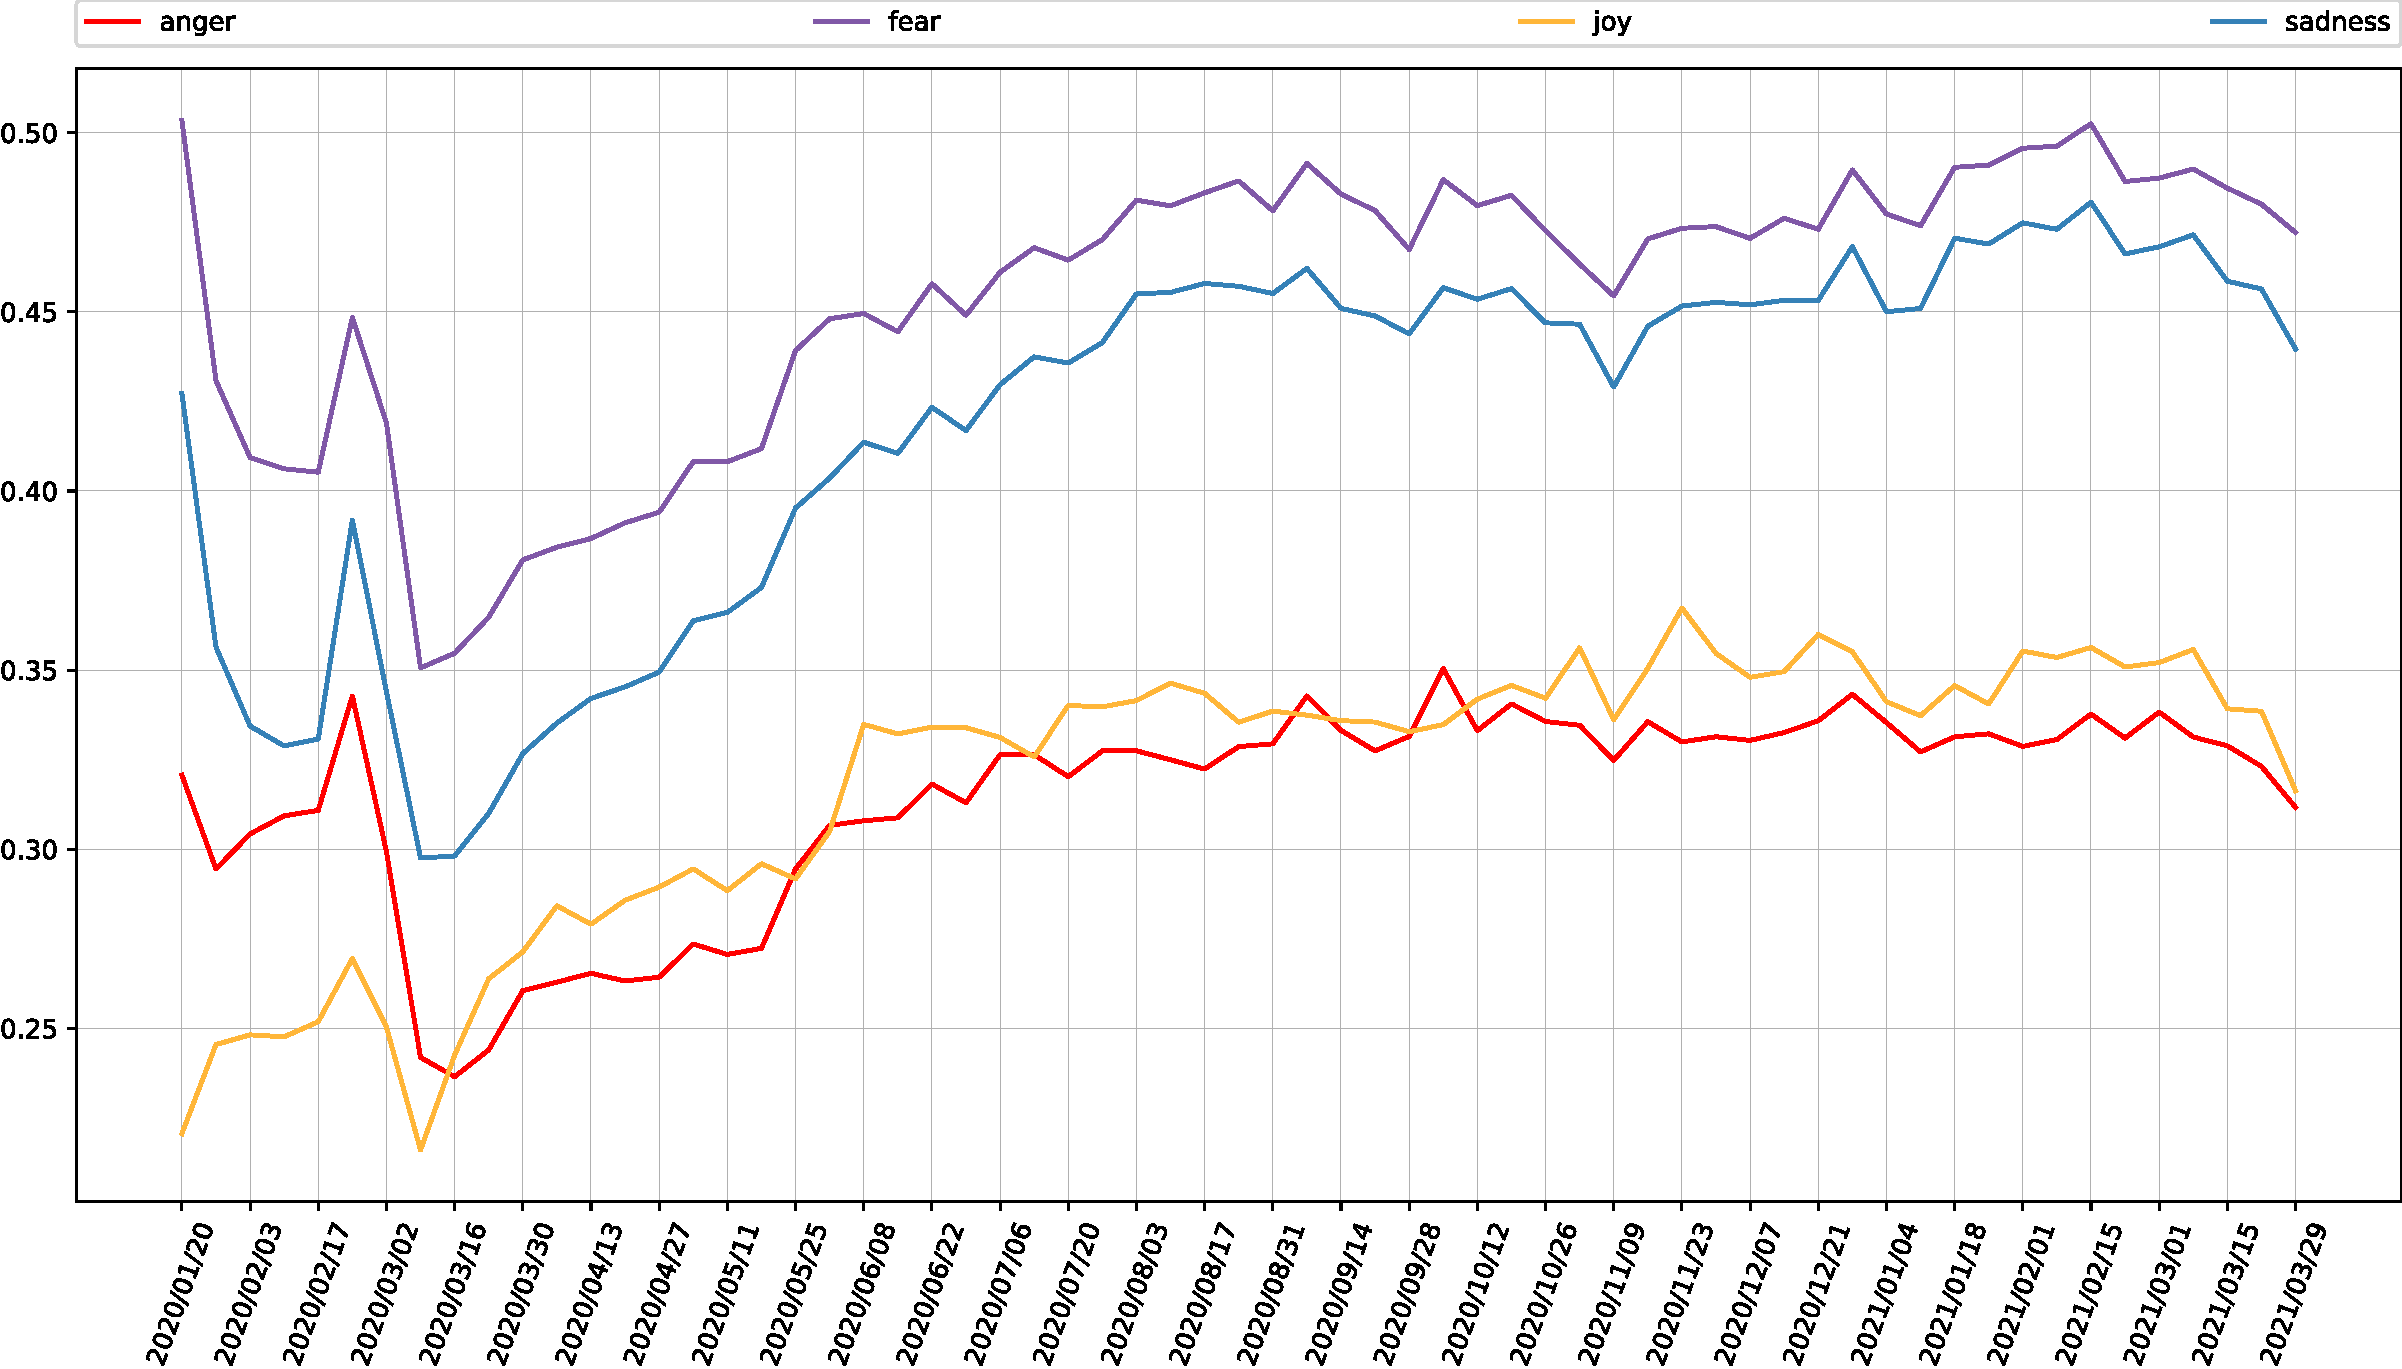
\includegraphics[scale=.35]{en_4_emotions.svg}
    	\caption{Proportion of weekly users per emotion in the English tweets}
    	\label{fig:en-4-emotions}
\end{figure}

\Cref{fig:en-4-emotions} instead shows the proportion of users that expressed a particular emotion in a given week, considering the English tweets. Here we can notice some interesting results: first of all, there are some cases where all the emotions seem to have the same course. We would have expected that, if negative emotions increased, positive emotions would decrease (and vice versa). Instead, during the week starting on 2020/02/24, the proportion of users that expressed anger, joy, fear, and sadness raised. This probably happened because users during that time were particularly emotional and used several more words within a tweet. However, that is not always the case: for example, during 2020/07/13 the joy decreased, while fear, and sadness increased.

Secondly, it is also possible to observe how time frames of greater joy alternate with periods of greater anger. However, that is not the case for fear and sadness. This probably happens because there are a lot of words that convey both these emotions at the same time. In practice, when one increases, so does the other.

\begin{figure}[H]
	\centering
    	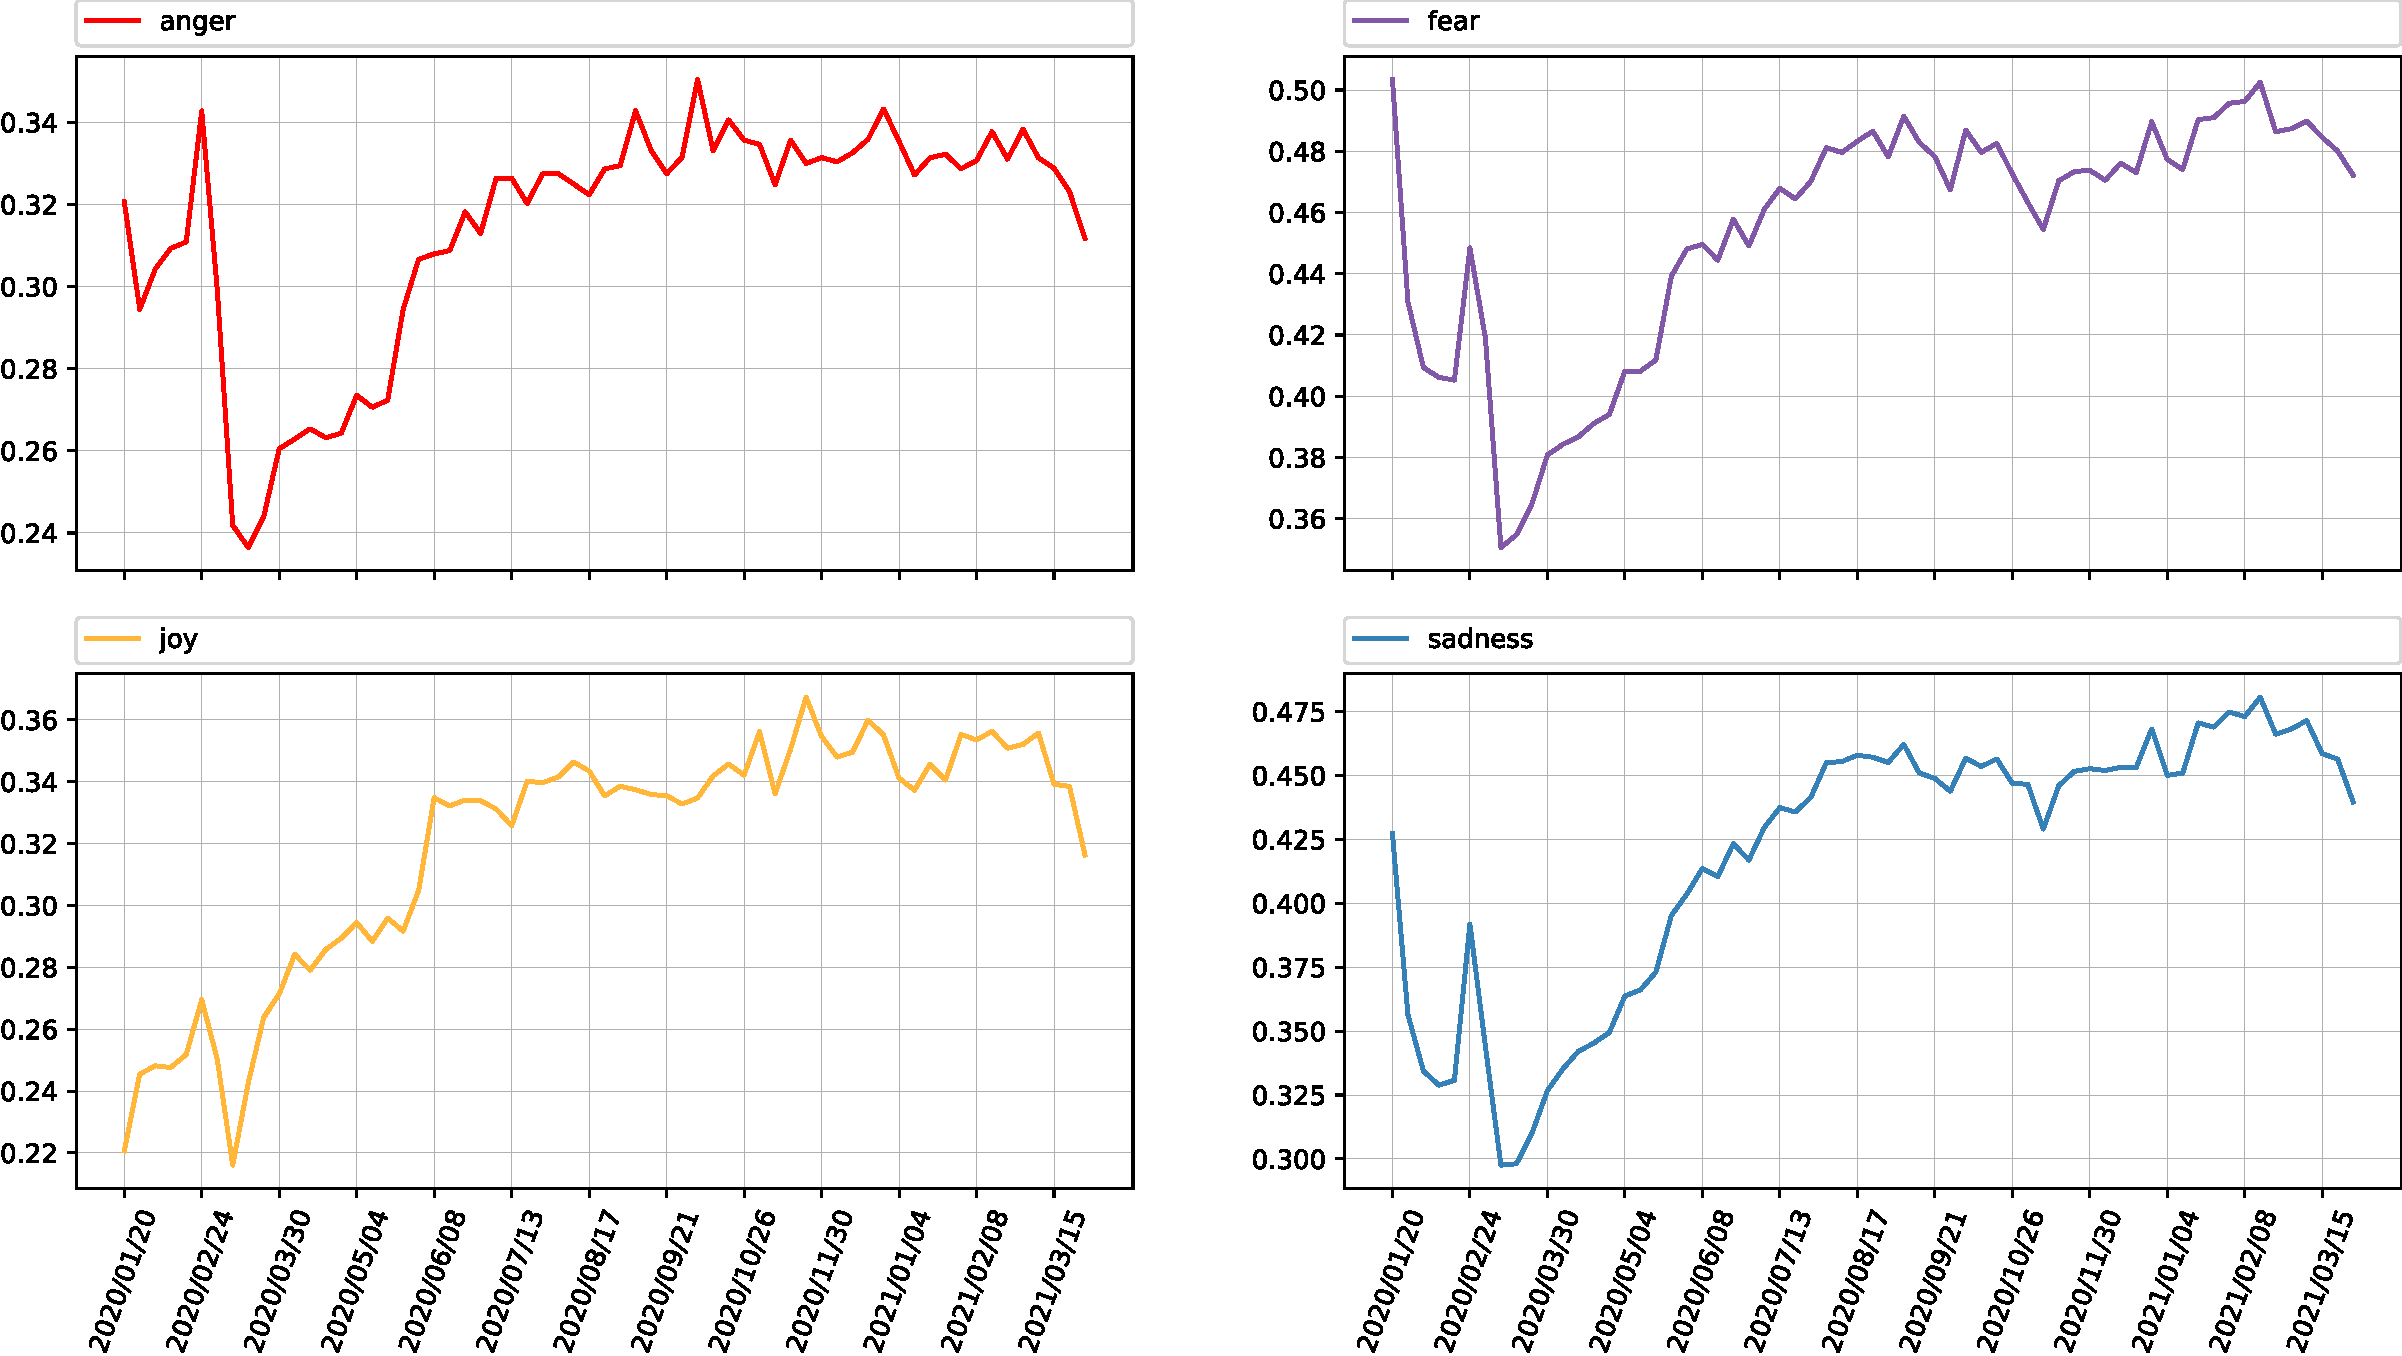
\includegraphics[scale=.35]{en_4_emotions_subplot_1.svg}
    	\caption{Proportion of weekly users expressing a particular emotion in the English tweets}
    	\label{fig:en-4-emotions-subplot-1}
\end{figure}

Before approaching the data normalization, we have also tried to divide the different emotions courses into subplots. If we take a look at \Cref{fig:en-4-emotions-subplot-1}, both global (and local) maxima and minima are visible to the naked eye. However, the comparison between different emotions becomes really difficult.

\begin{figure}[H]
	\centering
    	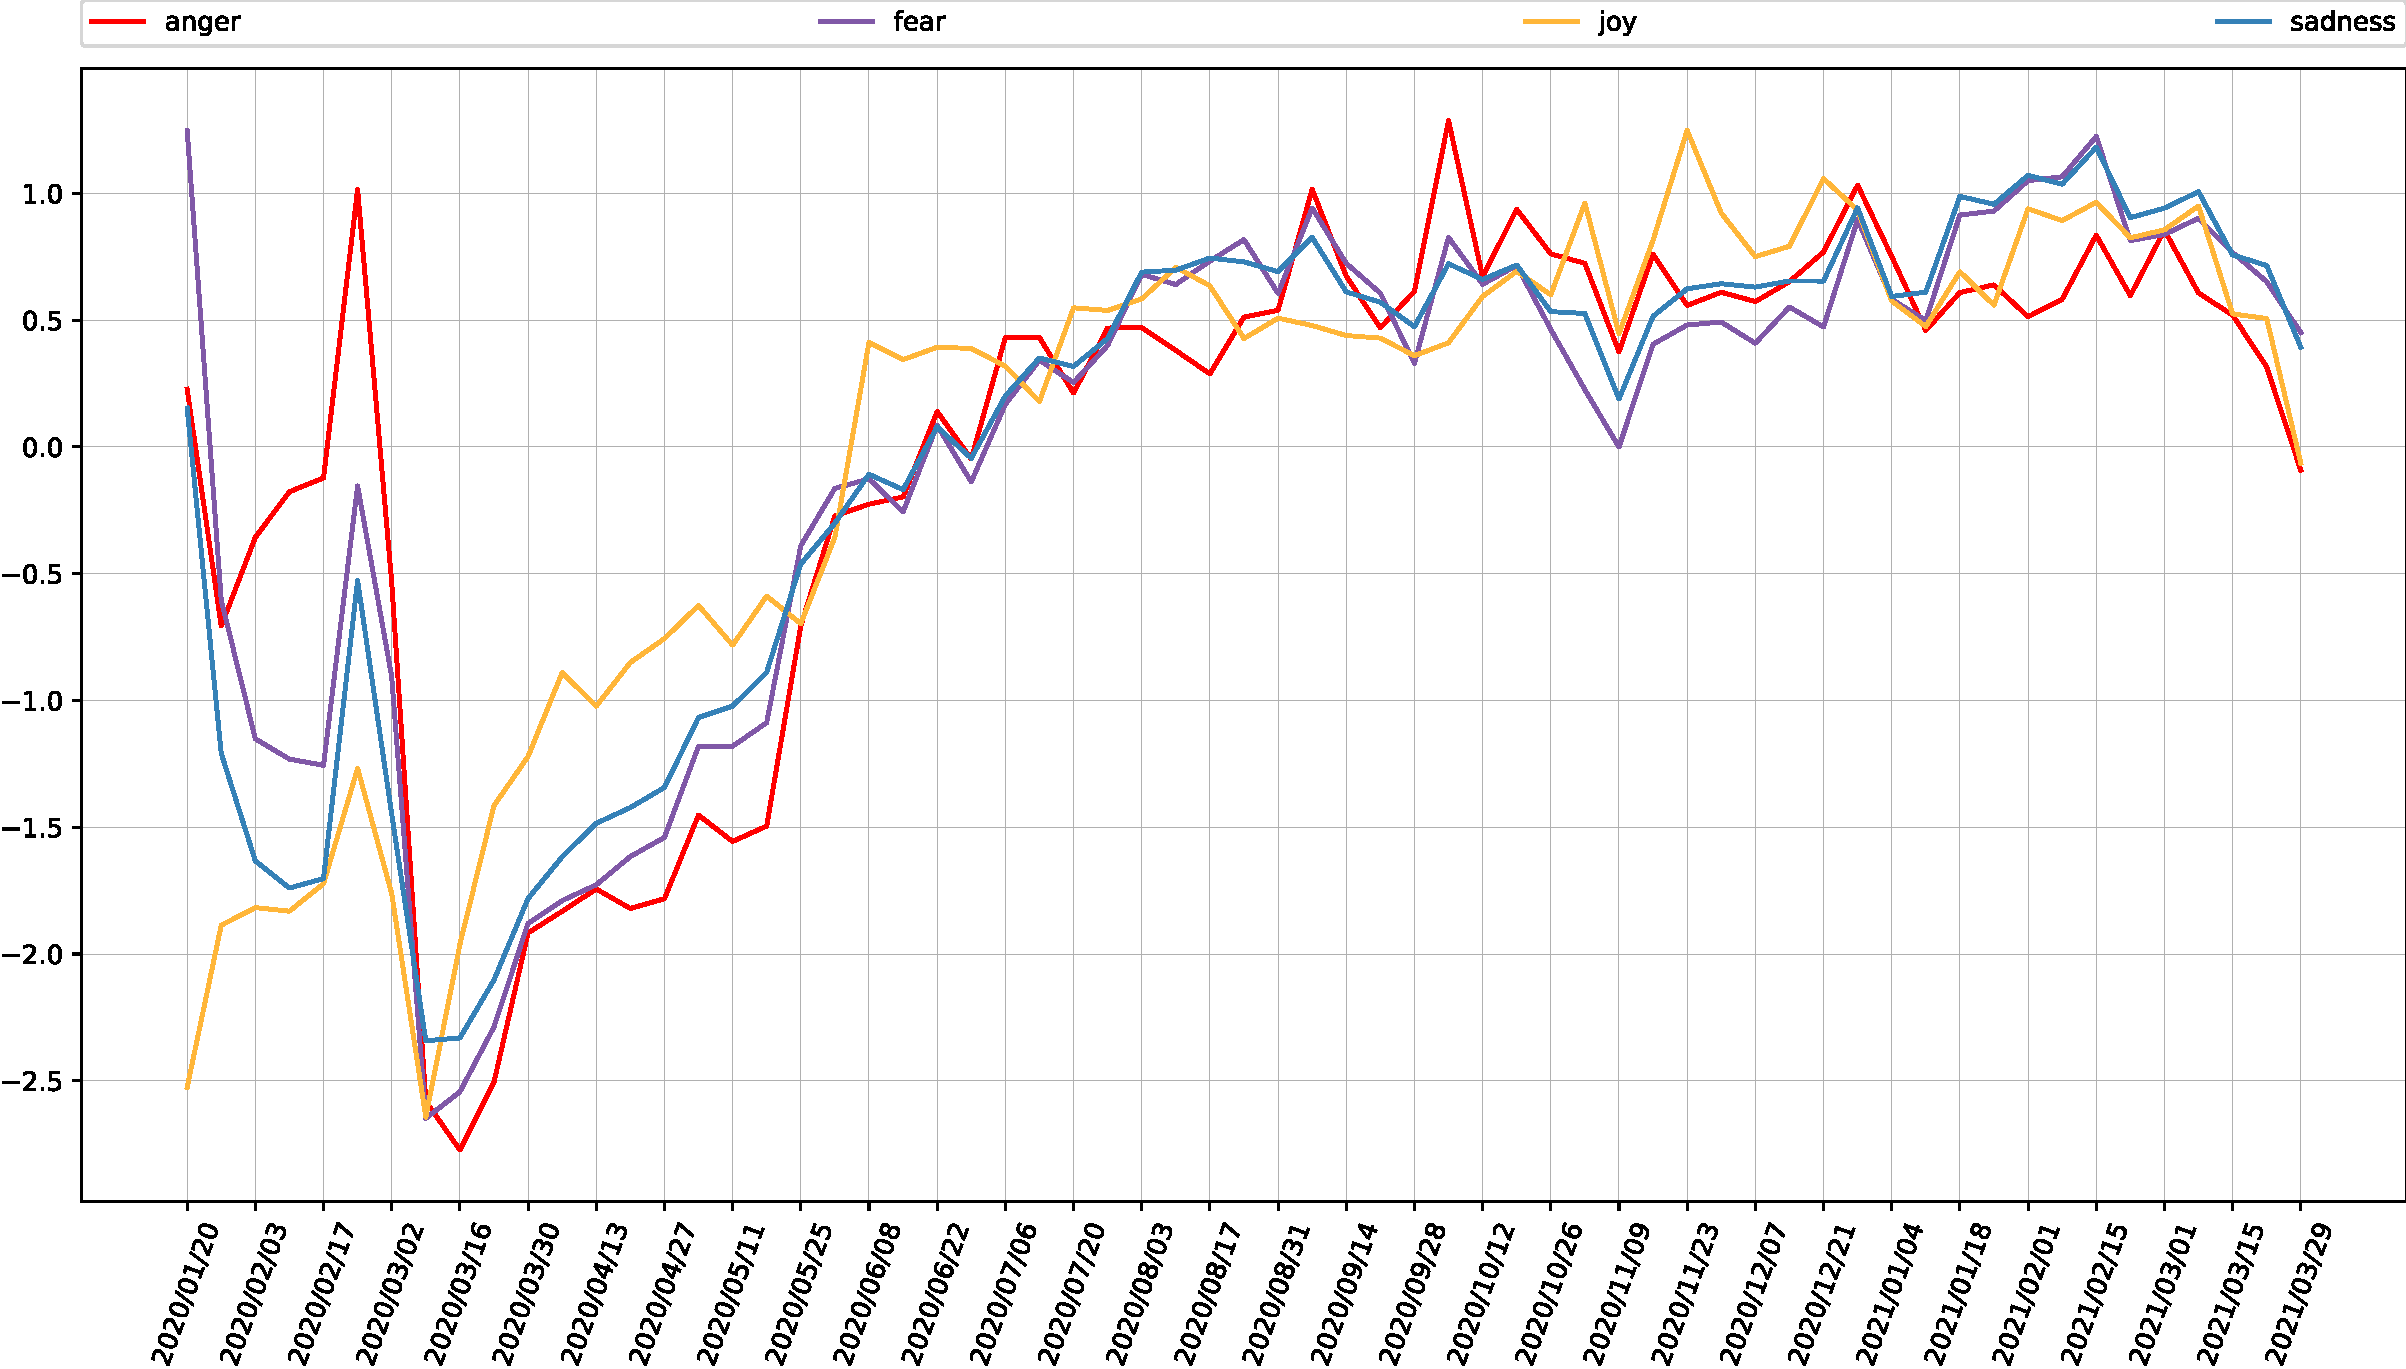
\includegraphics[scale=.35]{en_4_emotions_standardized.svg}
    	\caption{Z-score of weekly users per emotion in the English tweets}
    	\label{fig:en-4-emotions-std}
\end{figure}

The z-score instead proved to be a very useful data normalization. As we can see from \Cref{fig:en-4-emotions-std}, not only peaks are noticeable even if we are considering the emotions altogether, but we can also understand which time frames are characterized by a greater (or lower) emotion value w.r.t. the mean value of that particular emotion. For example, it is possible to see that, starting on 2020/03/16, the proportion of users that expressed joy w.r.t. the mean value of joy over the whole period, surpassed all the other emotions w.r.t. their mean value over the whole period.

From the comparison of the course of the emotions we have selected some peaks (i.e. week) manually to understand which words were the most used. 

\begin{figure}[H]
	\centering
    	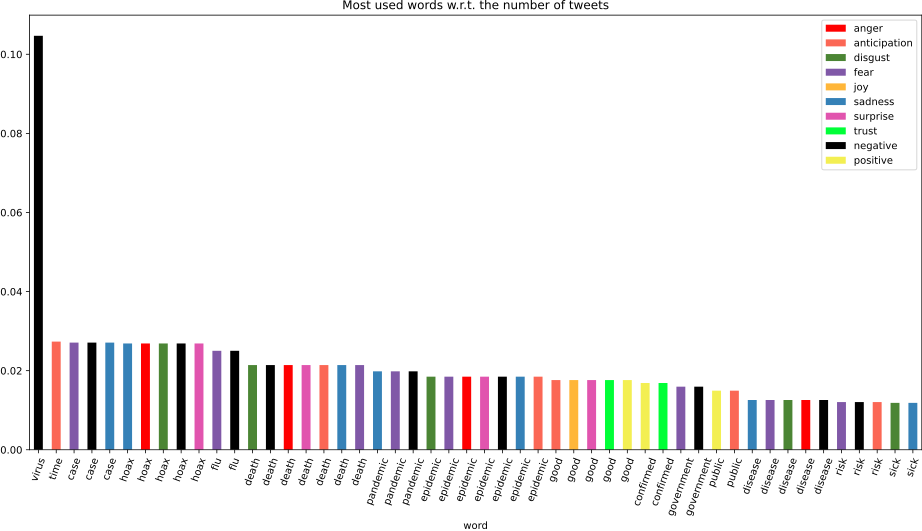
\includegraphics[scale=.35]{en_most_used_words_2020_02_24.svg}
    	\caption{Proportion of most used words on 2020/02/24 that express emotion/sentiment in the English tweets}
    	\label{fig:en-most-used-word-2020-02-24}
\end{figure}

\Cref{fig:en-most-used-word-2020-02-24} shows which are the 50 most used words in the English tweets during the week starting on 2020/02/24.

Here, we can see that some words, such as “virus”, are only related to a sentiment and not to any other emotion. On the other hand, “epidemic” is associated to almost the totality of the emotions.

It is also very interesting that the word “virus” was present in 10\% of the tweets. Moreover, we can also see that this particular graphics validates the previous hypothesis: indeed, there are lot of words that convey both sadness and fear. In particular, we can notice that it is the case for “case”, “death”, “pandemic”, “epidemic”, and “disease”.

\begin{figure}[H]
	\centering
    	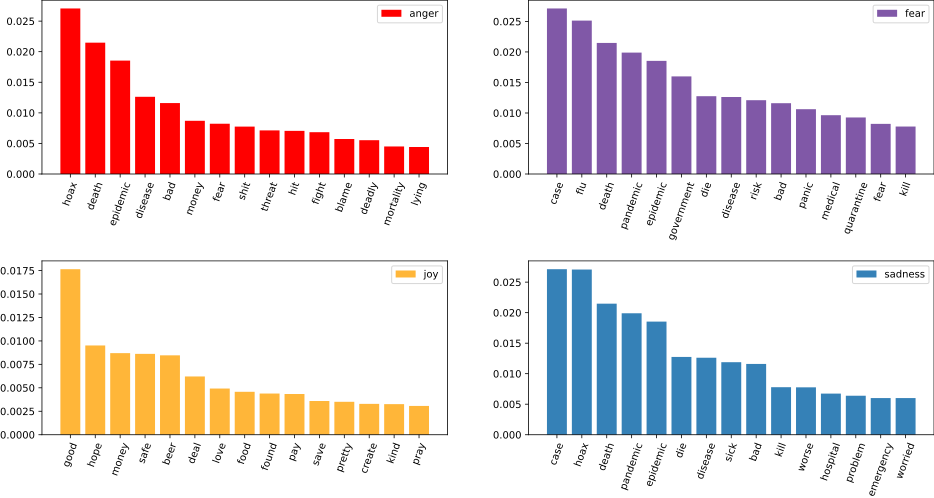
\includegraphics[scale=.35]{en_most_used_words_4_emotions_2020_02_24_subplot.svg}
    	\caption{Proportion of 15 most used words on 2020/02/24 per emotion in the English tweets}
    	\label{fig:en-most-used-word-subplot-2020-02-24}
\end{figure}

Instead, \Cref{fig:en-most-used-word-subplot-2020-02-24} shows the 15 most used words for anger, fear, joy, and sadness. if we look at the subplots of fear and sadness, we can clearly see that the tweets contain more words expressing fear than sadness. This explains once again the course of the emotions in \Cref{fig:en-4-emotions}.

\begin{figure}[H]
	\centering
    	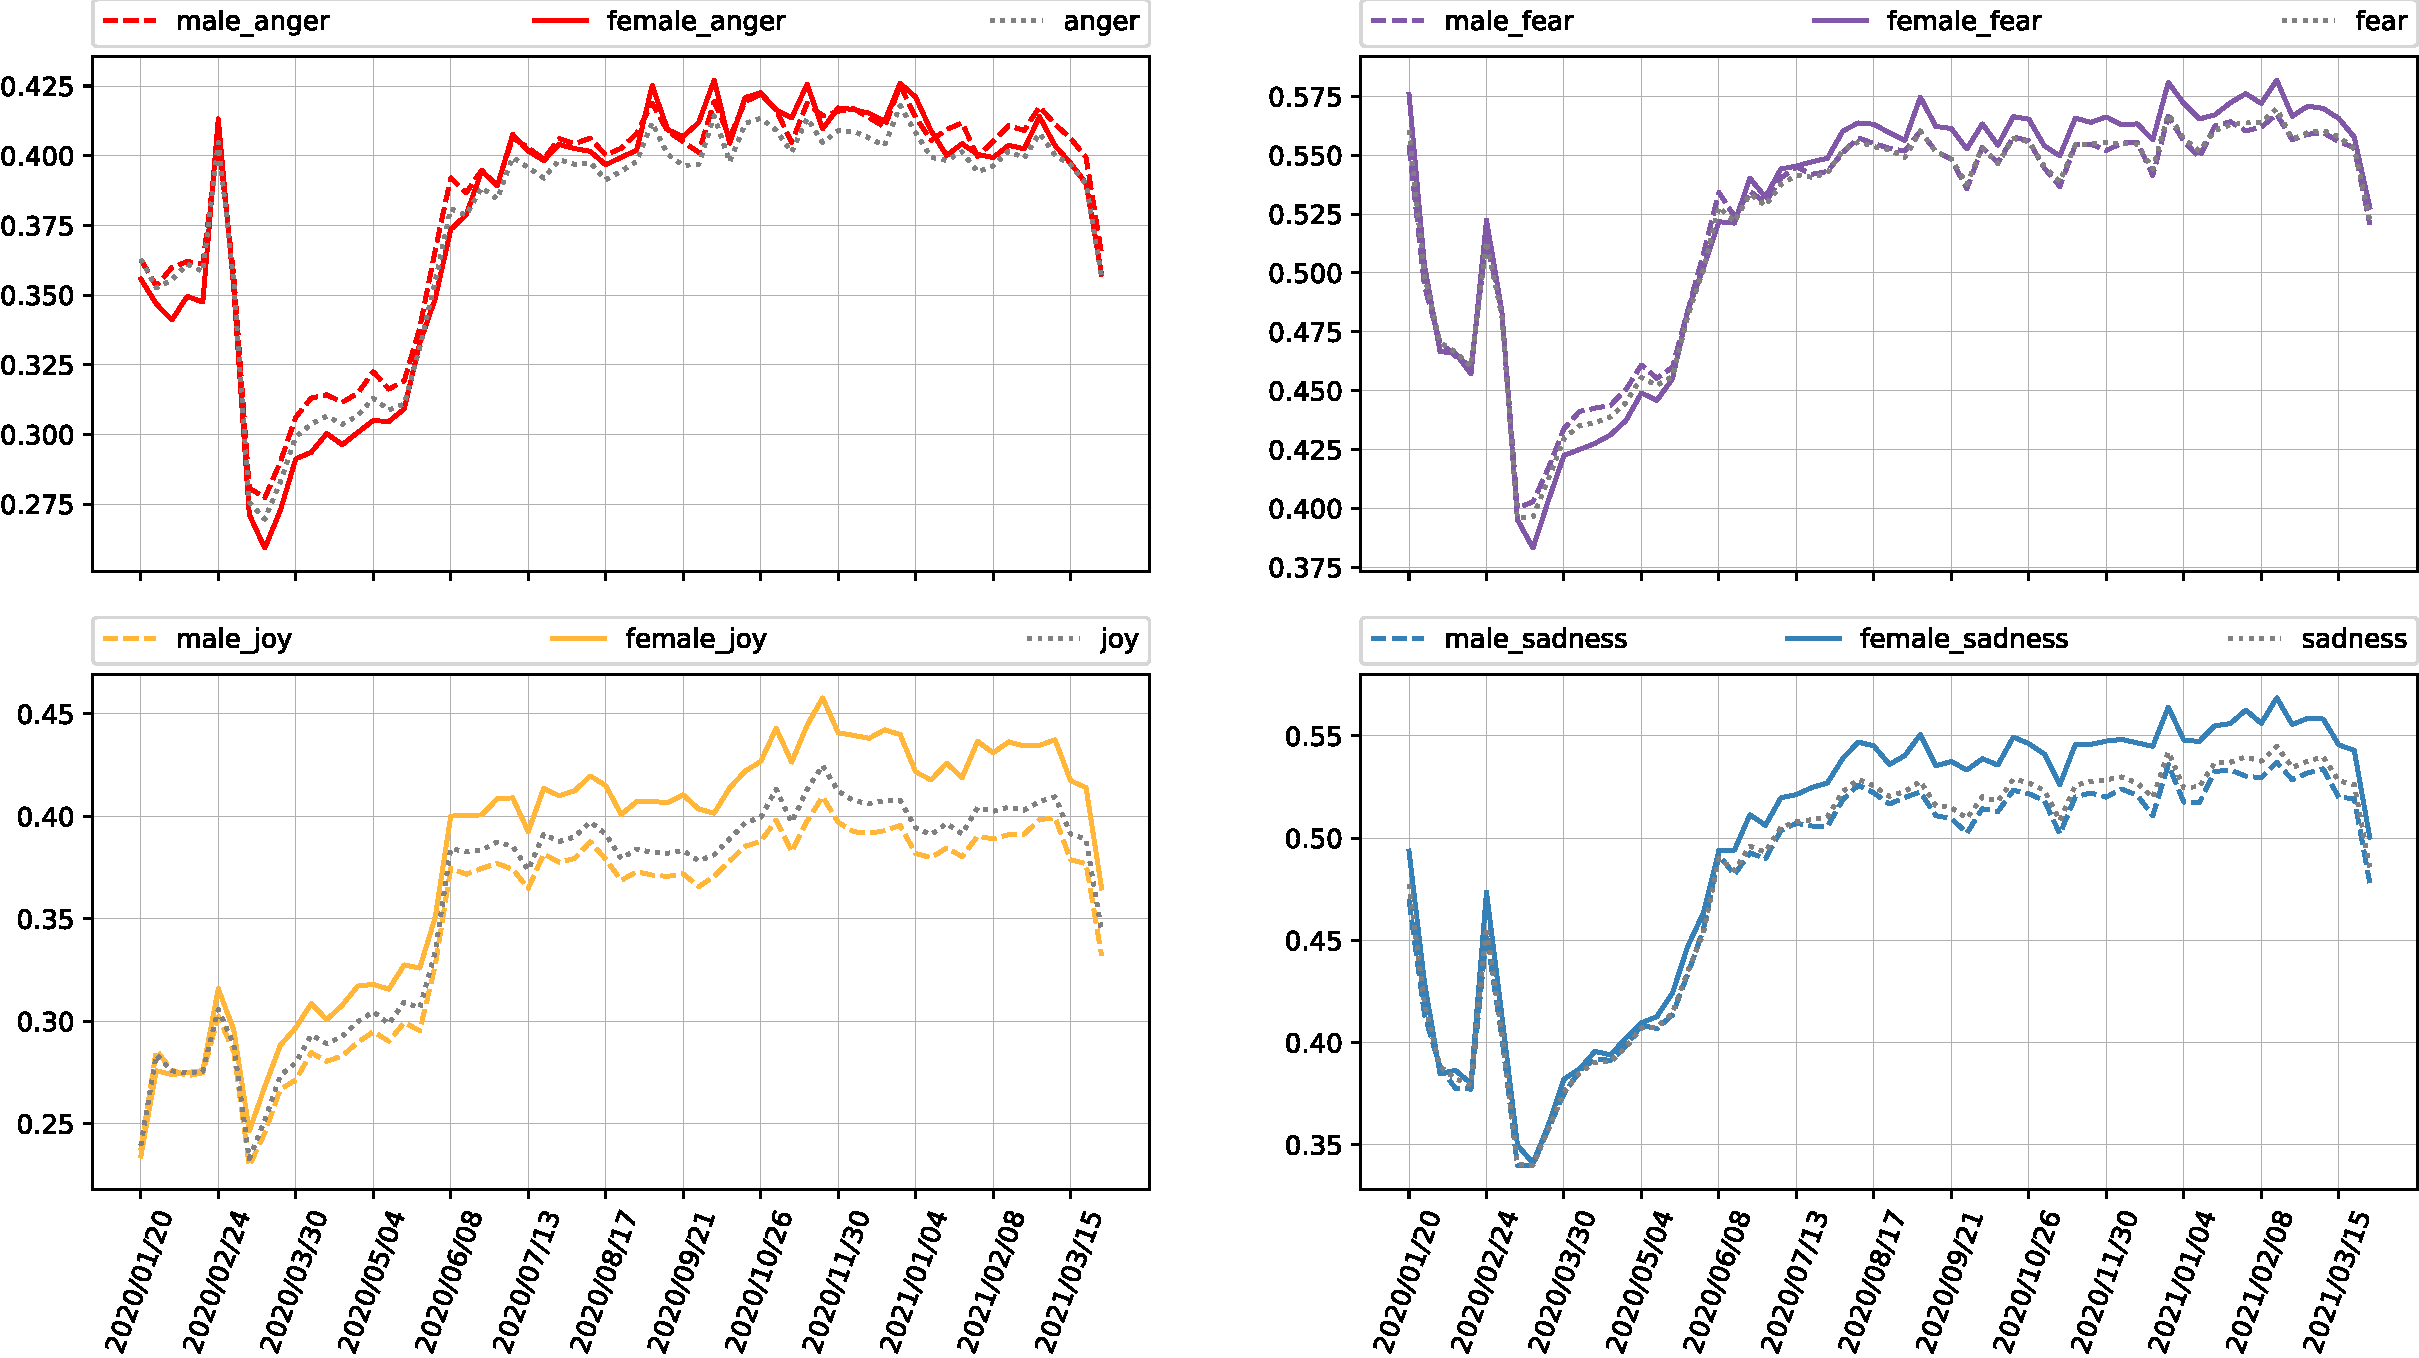
\includegraphics[scale=.35]{en_4_emotions_per_category_with_course_subplot_1.svg}
    	\caption{Proportion of weekly men/women expressing a particular emotion in the English tweets}
    	\label{fig:en-4-emotions-per-category-course-subplot-1}
\end{figure}

\Cref{fig:en-4-emotions-per-category-course-subplot-1} introduces the results of the analysis of the emotions expressed by females and males in the English tweets during the whole period. In this case, the dotted gray line represents the proportion of users that, independently from the category they belong to, expressed a certain emotion on a given week. However, this line differs from the results obtained in \Cref{fig:en-4-emotions-subplot-1}, because we are now considering only the users with a certain number of tweets (see \Cref{subsec:m3inference} for further details).

We can also see that women tend to write a lot more tweets that convey joy in most cases. This seems to be also the case for sadness and fear. However, if we consider for example the fear, the gap is very small. Instead, men seem to express slightly more anger over the considered period, but the two lines mostly overlap.

\begin{figure}[H]
	\centering
    	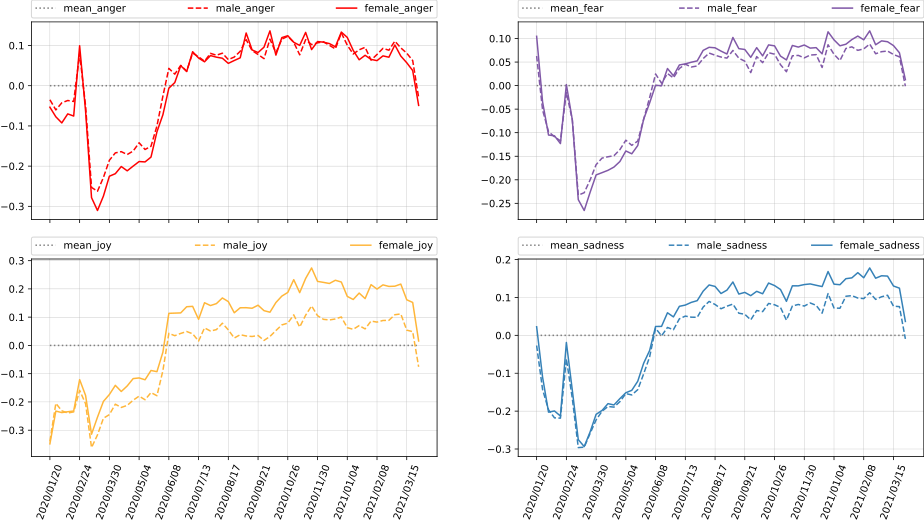
\includegraphics[scale=.35]{en_4_emotions_per_category_over_mean_subplot_1.svg}
    	\caption{Men/Women expressing the weekly proportion of a particular emotion w.r.t. the average value among all users}
    	\label{fig:en-4-emotions-per-category-course-mean-1}
\end{figure}

\Cref{fig:en-4-emotions-per-category-course-mean-1} is a variation of \Cref{fig:en-4-emotions-per-category-course-subplot-1}, where the gray dotted line indicates the average value of a particular emotion expressed by all the users (i.e. independently from the category) over the whole period. Instead, the proportion reported by the other lines represents how much a certain gender expressed a particular emotion in a given week w.r.t. the mean value among the users. For example, both males and females expressed 10\% more anger during the week starting on 2020/02/24.

\begin{figure}[H]
	\centering
    	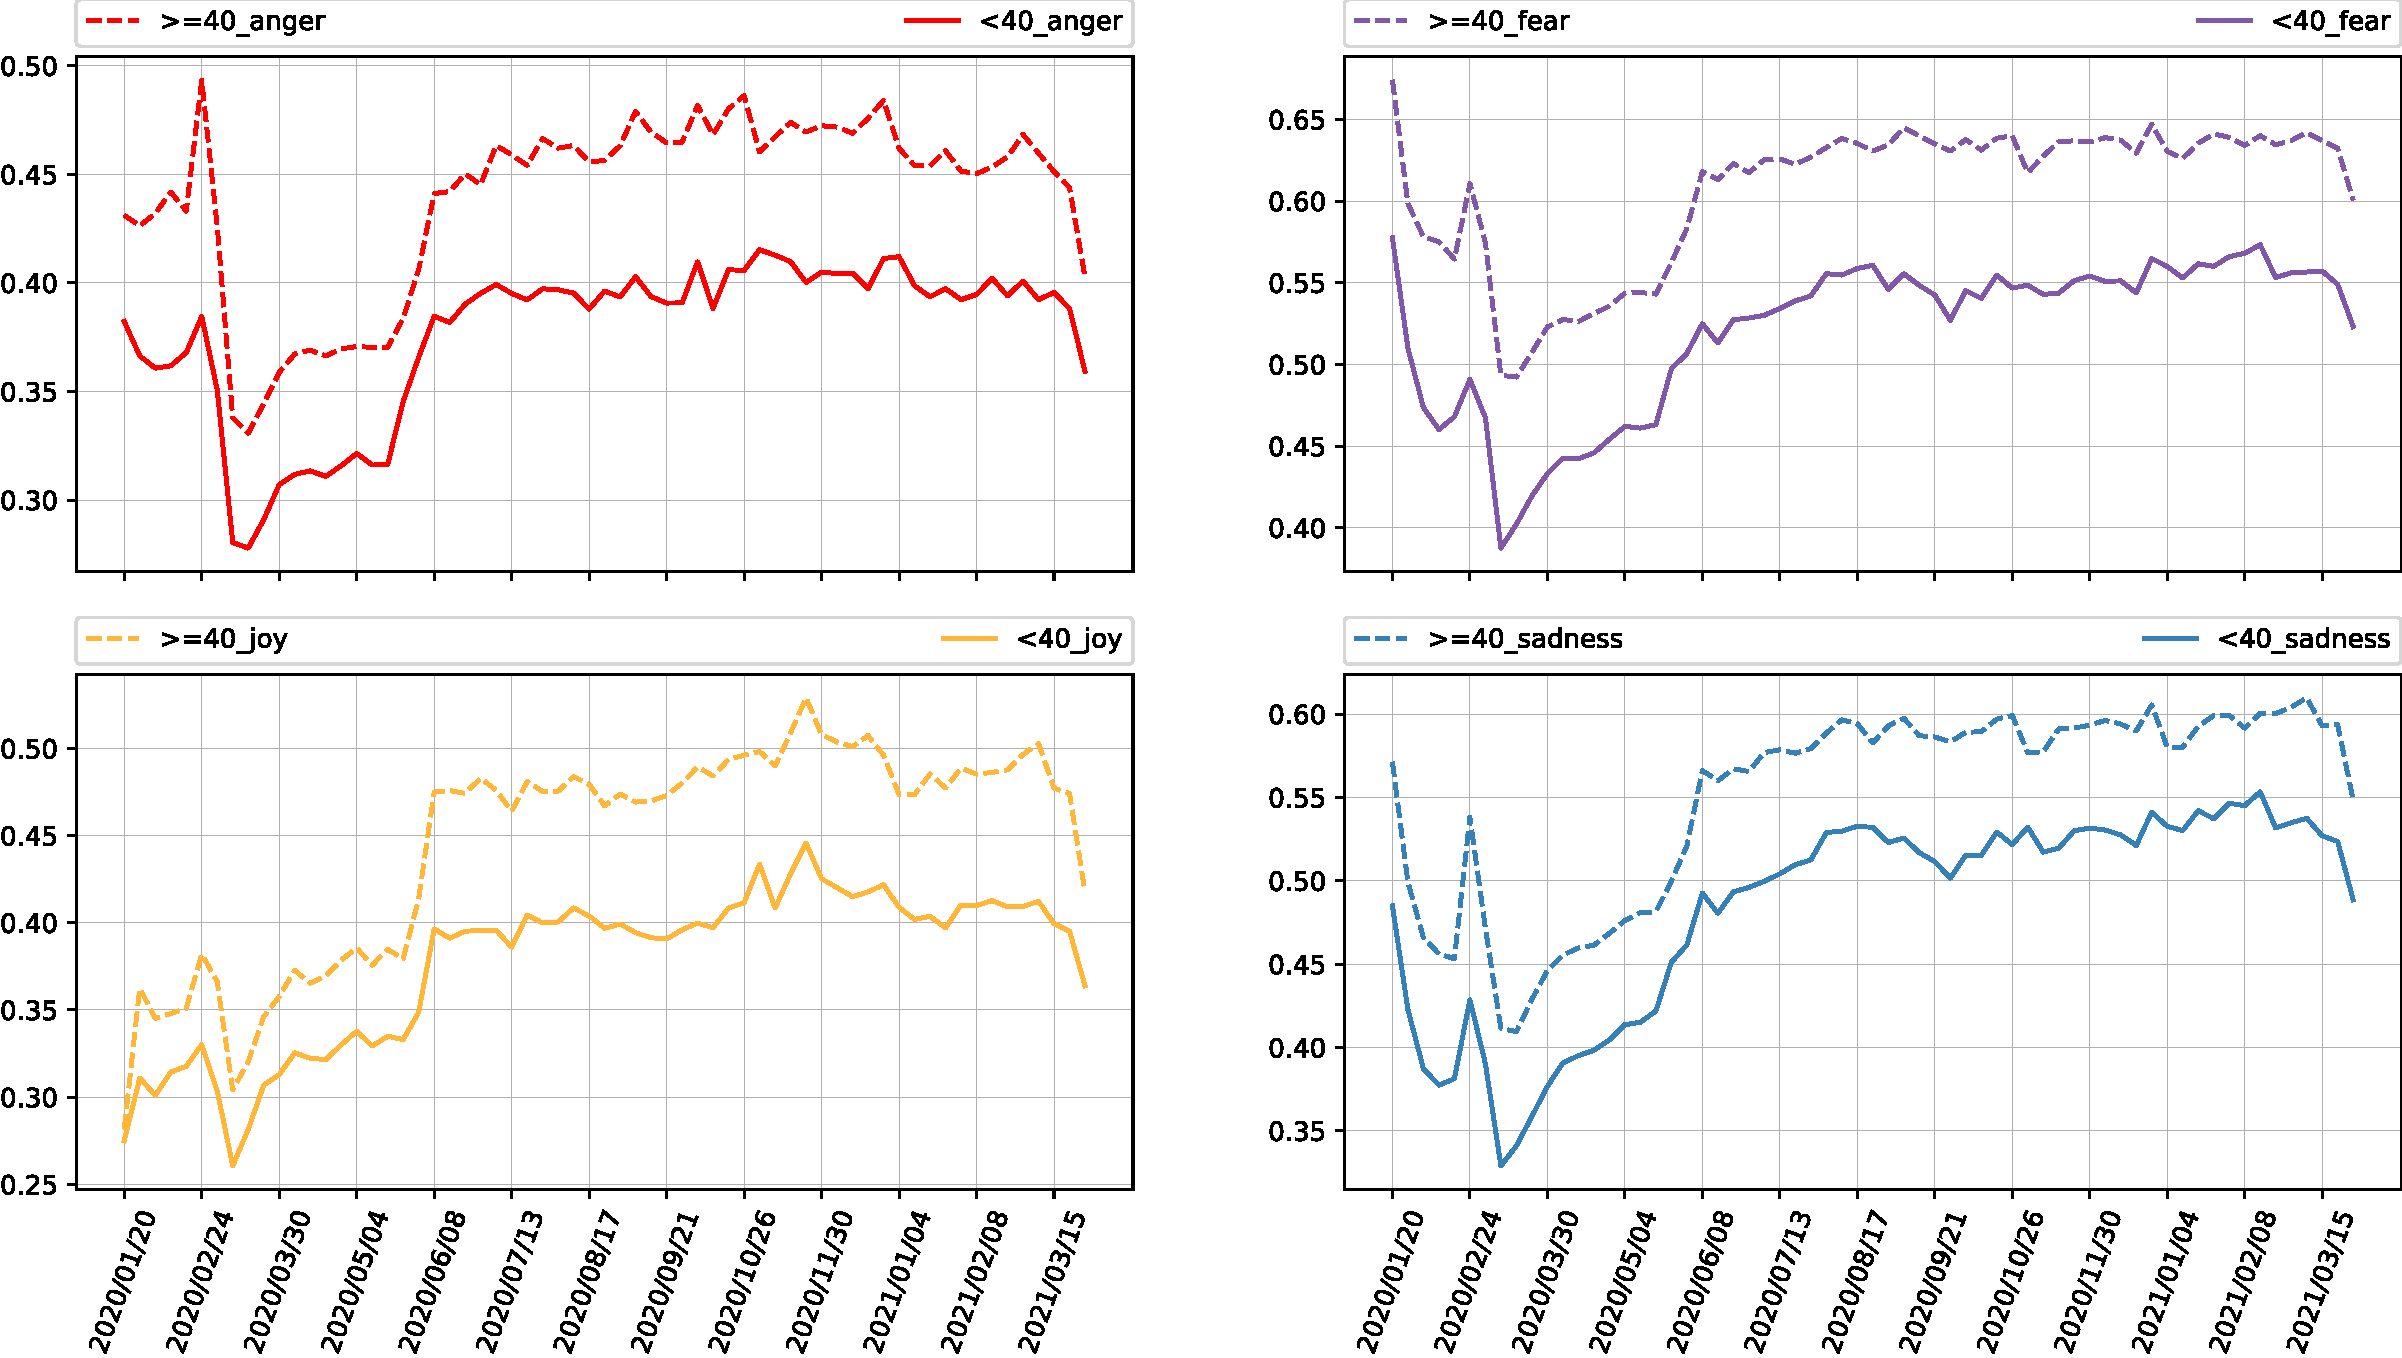
\includegraphics[scale=.35]{en_4_emotions_per_age_subplot_1.svg}
    	\caption{Proportion of weekly users per age expressing a particular emotion in the English tweets}
    	\label{fig:en-4-emotions-per-age-subplot-1}
\end{figure}

From the inference process, we also got information about age brackets. \Cref{fig:en-4-emotions-per-age-subplot-1} shows the course of the emotions per age for the considered period. The results obtained are very intriguing because there is always a noticeable gap between users with less than forty years and those with at least forty years. In particular, it seems that the ones belonging to the second age bracket are more inclined to convey their feelings.

\begin{figure}[H]
	\centering
    	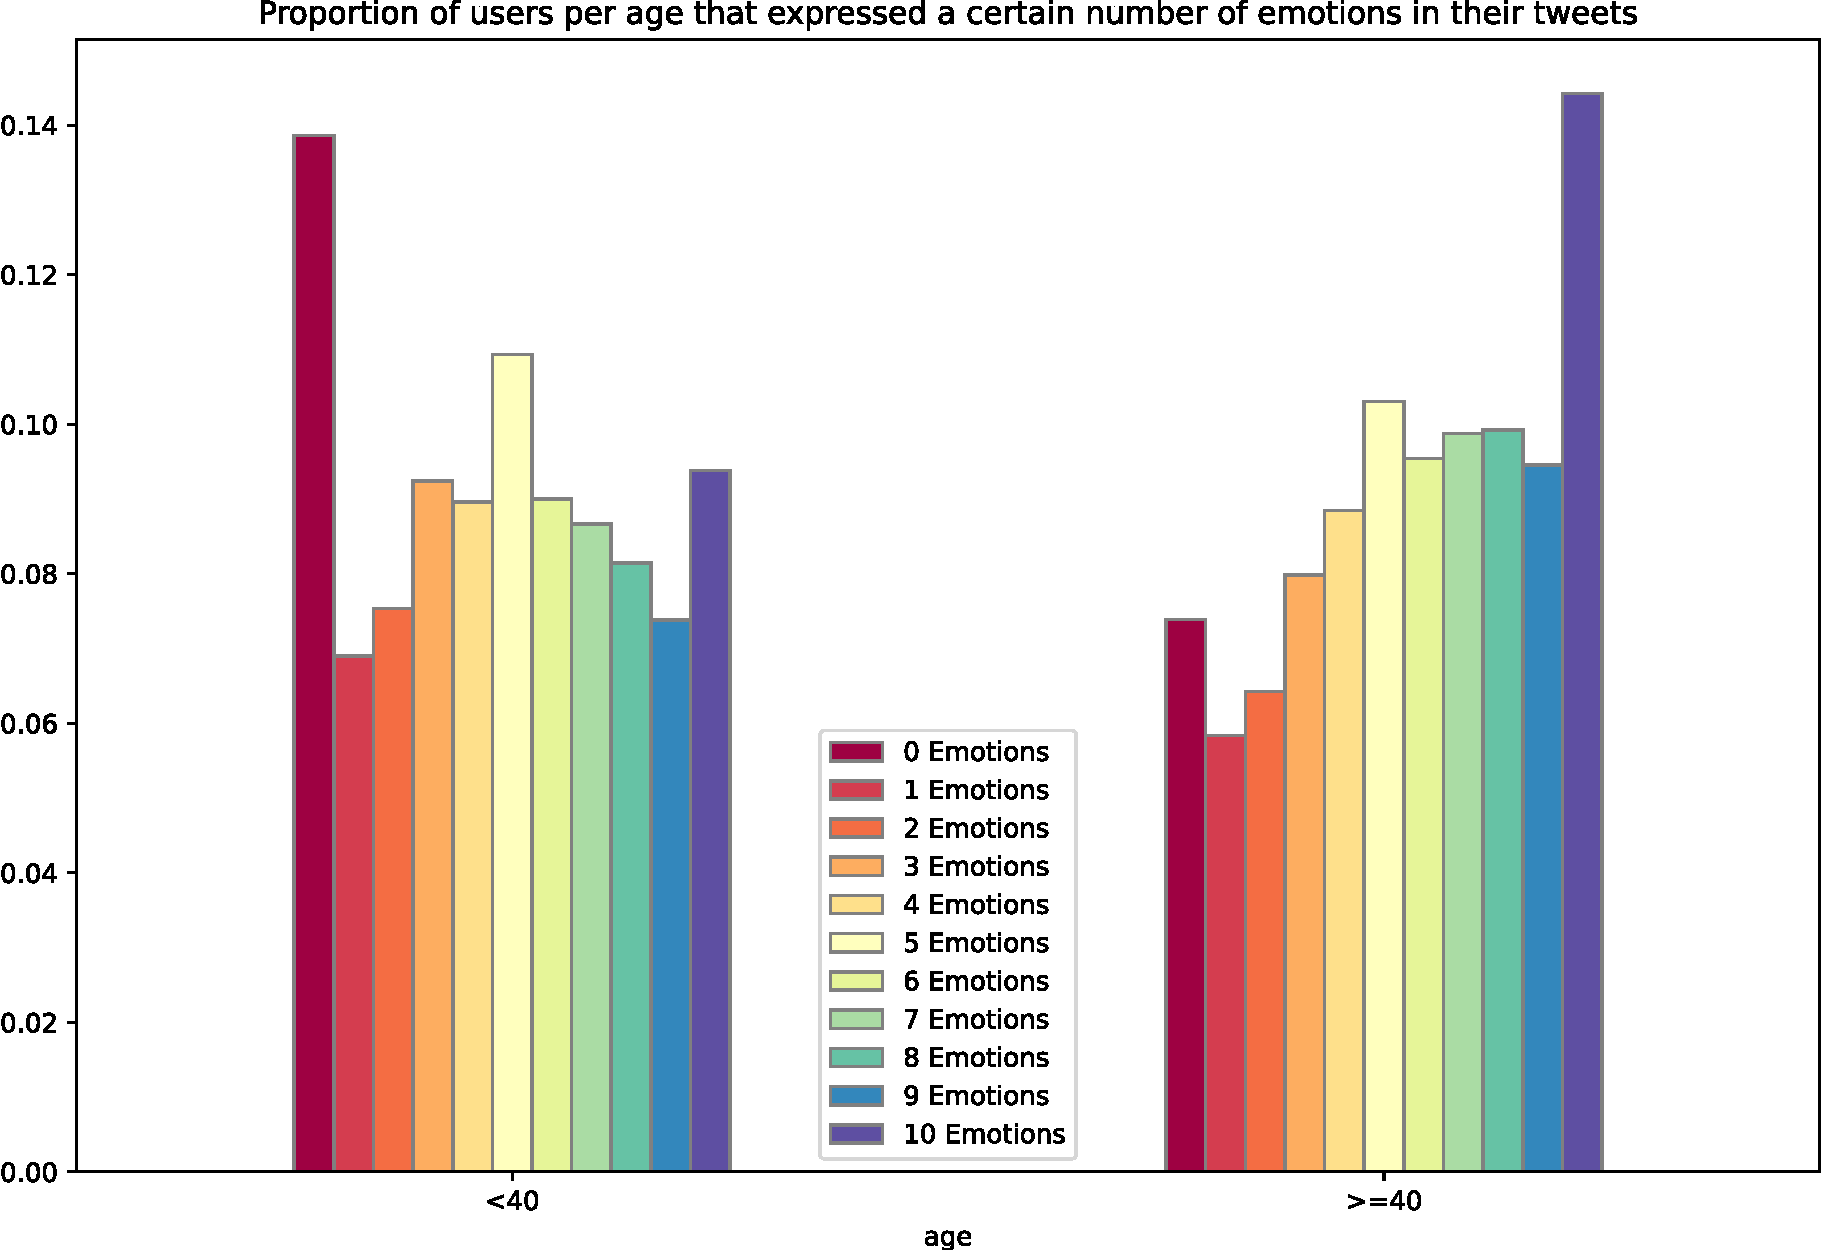
\includegraphics[scale=.35]{en_number_of_emotions_per_age.svg}
    	\caption{Proportion of users per age expressing zero or more emotions/sentiments}
    	\label{fig:en-4-emotions-per-age-per-number}
\end{figure}

\Cref{fig:en-4-emotions-per-age-per-number} shows the proportion of users that, in a given week, expressed a certain number of emotions/sentiments. As we can see, \(14 \%\) of the users with less than forty years did not express any emotion. This result is very interesting and could be caused by different reasons. For example, it may be possible that younger users like to write shorter tweets. In fact, with a very restricted set of words, it is likely to not express feelings at all. Besides, they could use different methods to convey their emotions, such through emoticons or slang: neither of them are in fact recognized by EmoLex. Finally, it could also be the case that they are apathetic. In any case, the fact that a great number of users with less than forty years did not express any emotion explains why there is such a large gap between the course of the emotions in \Cref{fig:en-4-emotions-per-age-subplot-1}.

\begin{figure}[H]
	\centering
    	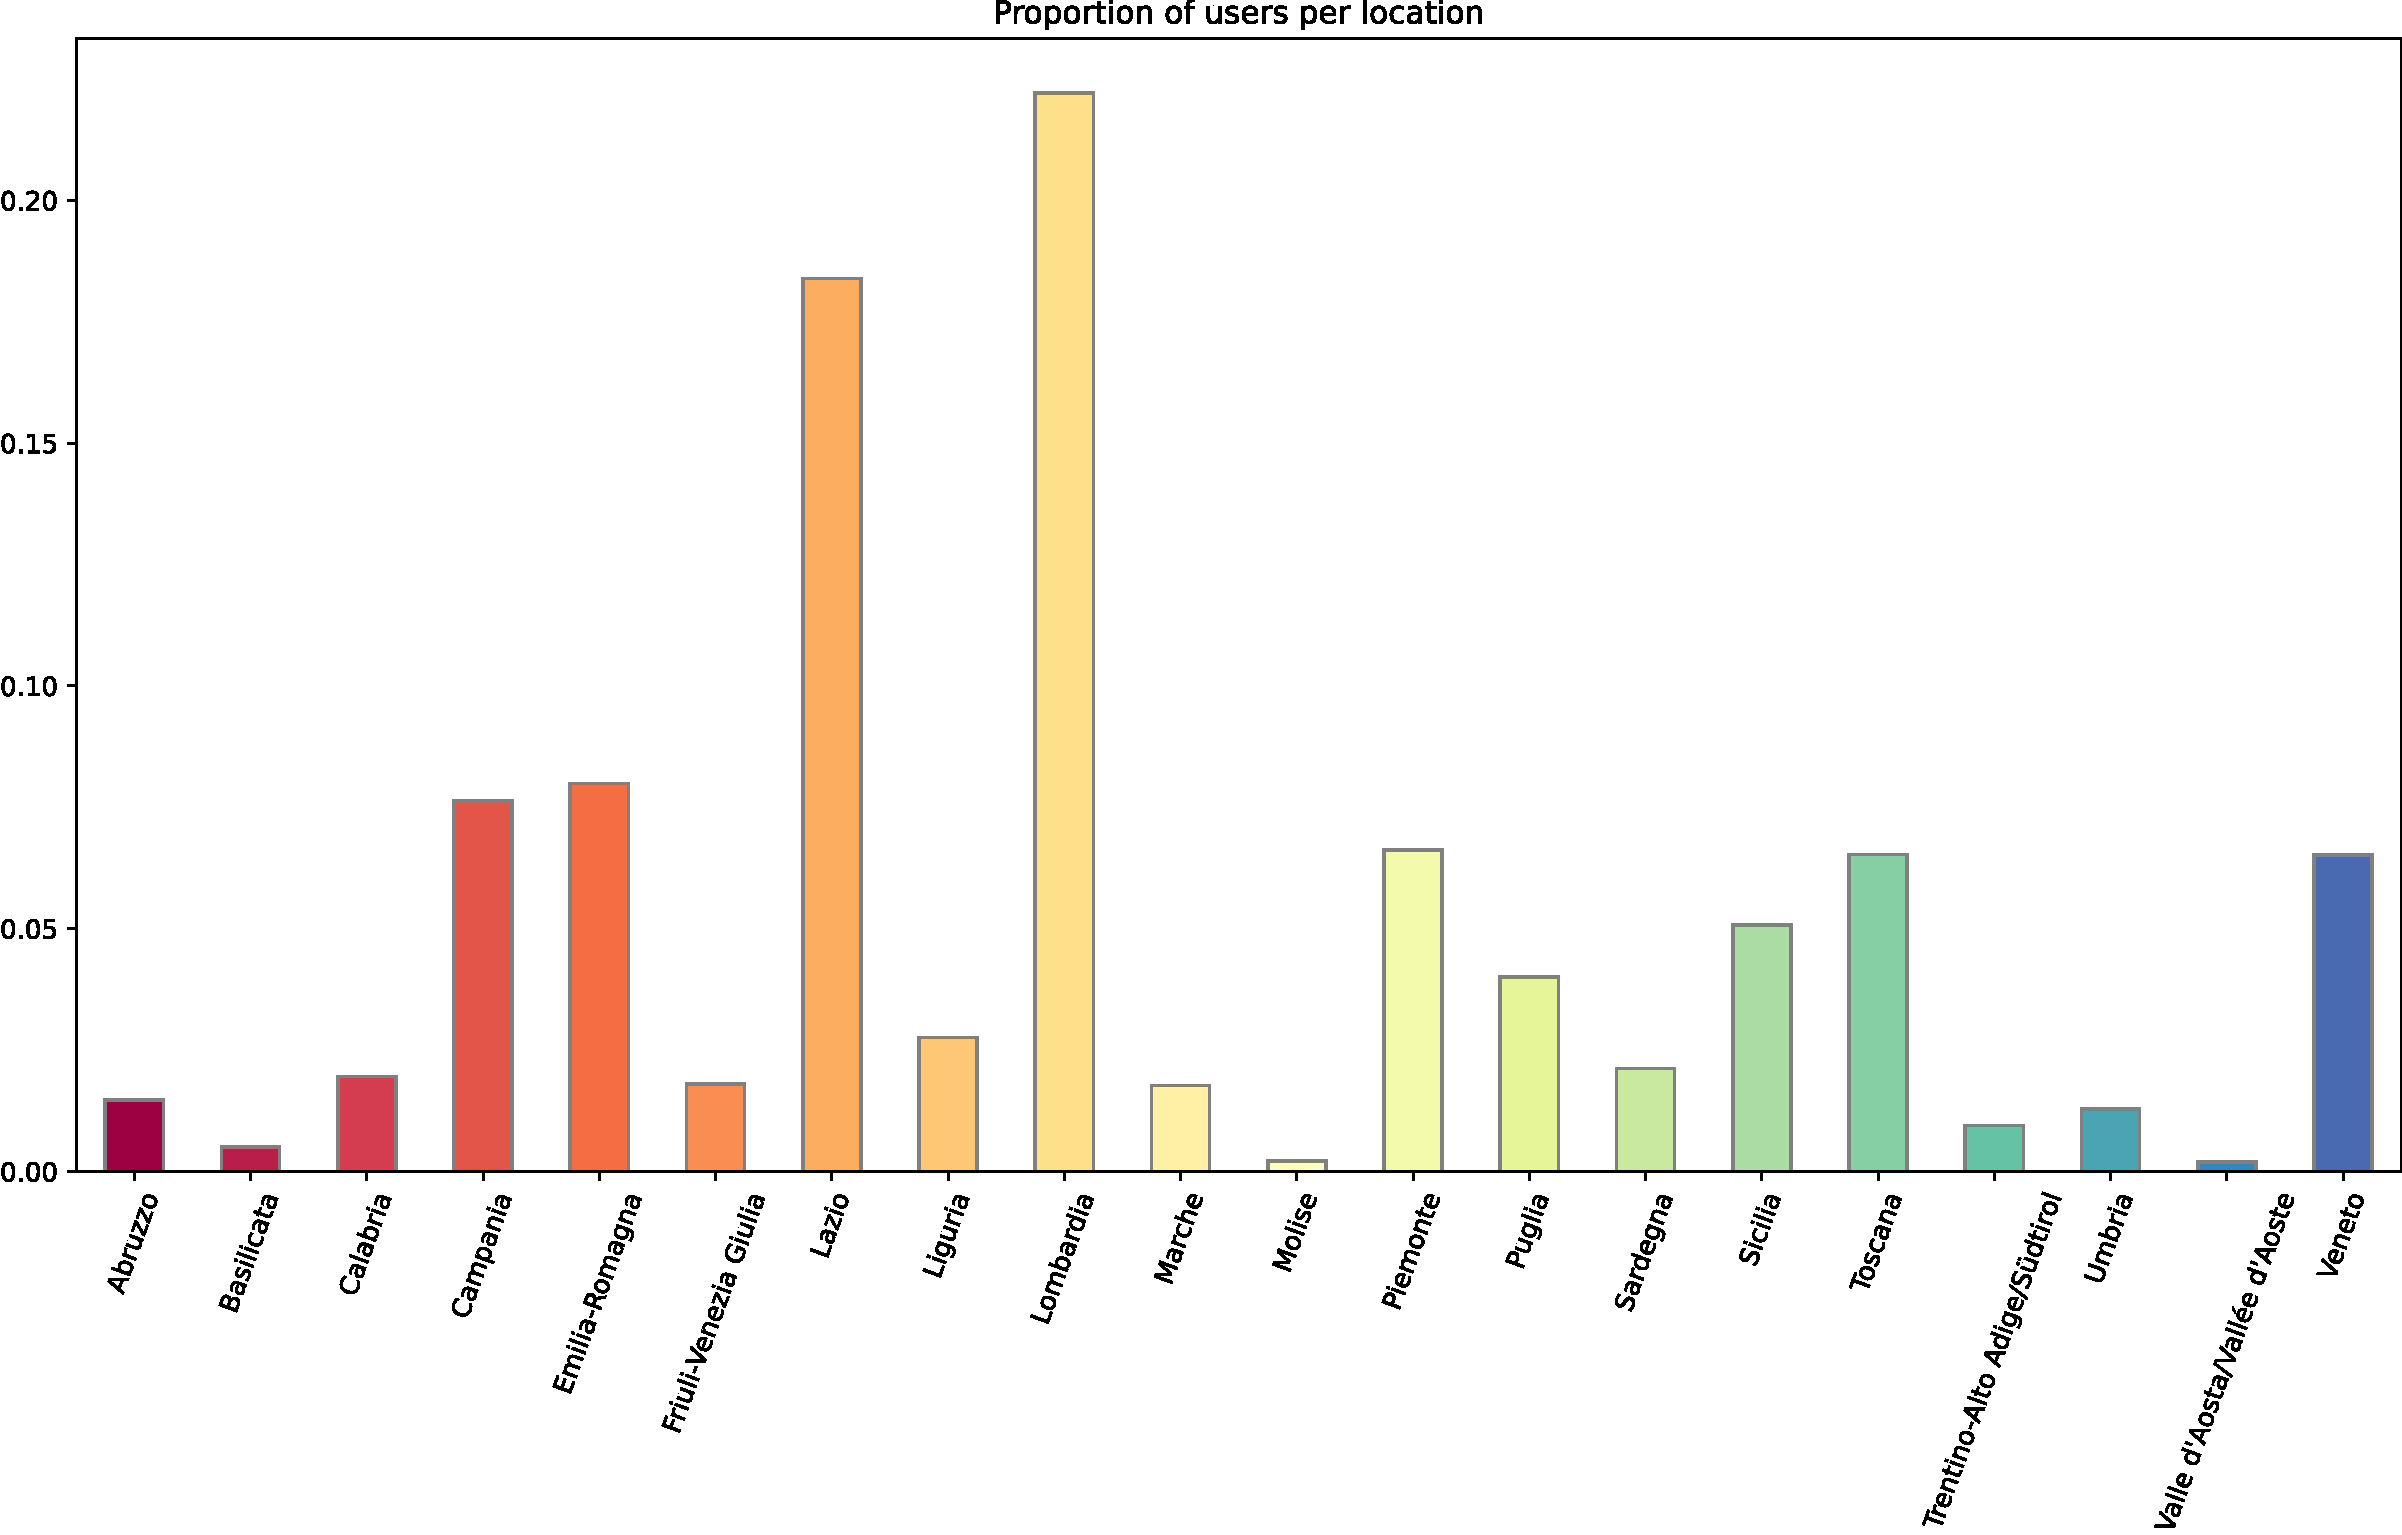
\includegraphics[scale=.35]{it_users_per_state.svg}
    	\caption{Proportion of users per state in Italy}
    	\label{fig:it-users-state}
\end{figure}

Finally, we can now move to the analysis of the users' emotions from a specific location. \Cref{fig:it-users-state} shows the proportion of users per state in Italy. From the results that we have obtained, we decided to consider only Lombardia, Lazio, Emilia Romagna, and Campania for further studies. In this way, we are able to better visualize the data and we have more possibilities to get stabler results. 

\begin{figure}[H]
	\centering
    	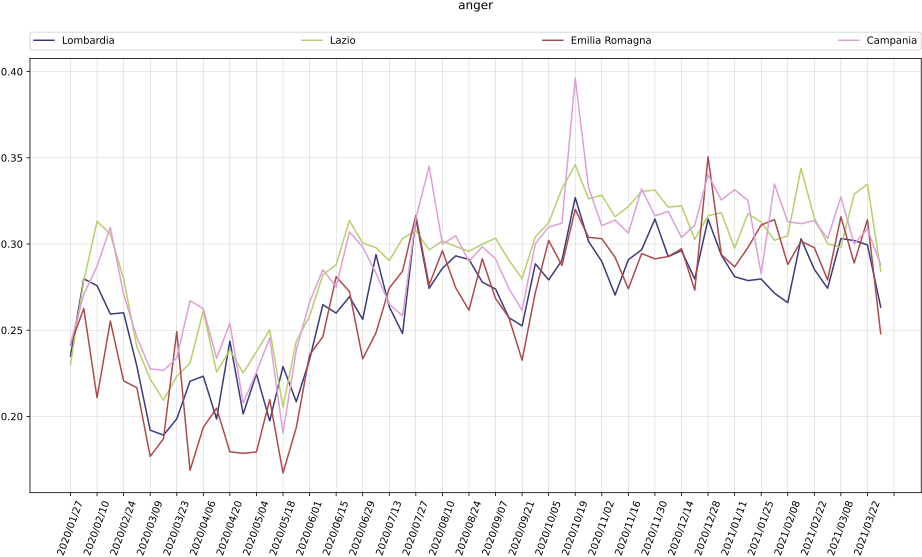
\includegraphics[scale=.35]{it_anger_4_states.svg}
    	\caption{Proportion of weekly users that expressed anger in Lombardia, Lazio, Emilia Romagna and Campania}
    	\label{fig:it-anger-4-states}
\end{figure}

From \Cref{fig:it-anger-4-states} we can actually understand which events had an impact on every state. For example, it is possible to notice a peak of anger on the week starting on the 2020/10/19. Here it is a bit more difficult to understand what actually happened without more complex techniques. However, from the analysis of the news, it is possible to link that particular time frame with the first of a series of different decrees, issued to stop the spreading of the disease once more after the first lockdown. 

\begin{figure}[H]
	\centering
    	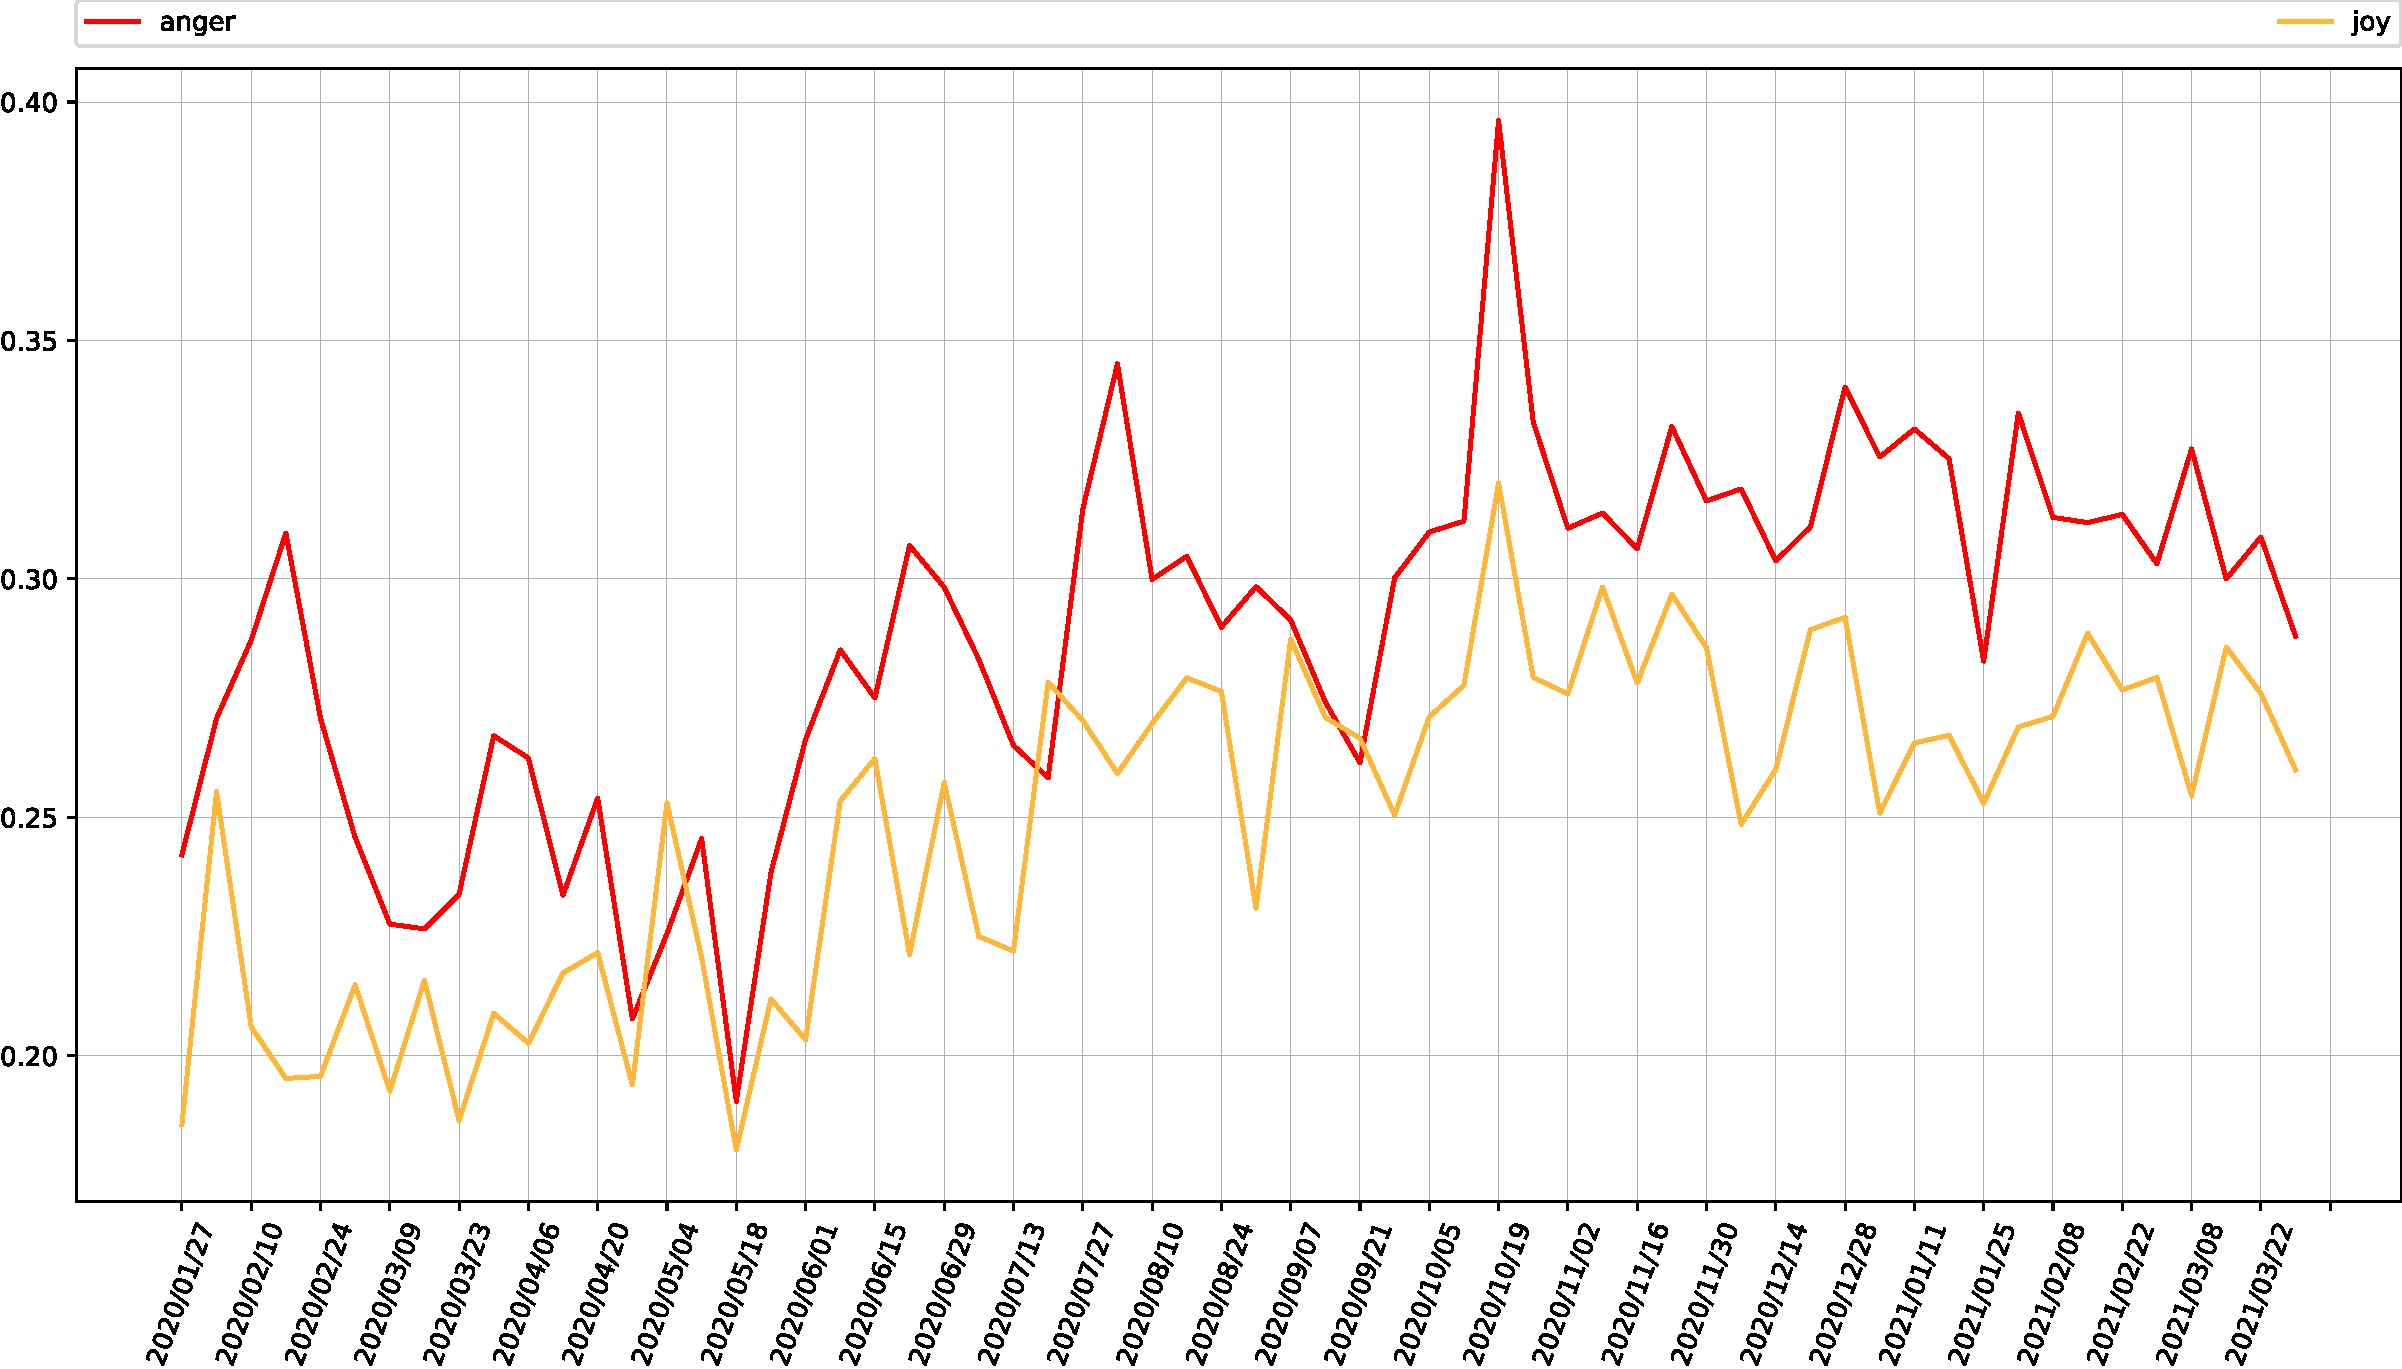
\includegraphics[scale=.35]{it_2_emotions_Campania.svg}
    	\caption{Proportion of weekly users that expressed anger and joy in Campania}
    	\label{fig:it-2-emotions-campania}
\end{figure}

Of course, it is also possible to consider a single state, for example Campania, as showed in \Cref{fig:it-2-emotions-campania}. Here we can notice even more how, by looking at the week starting on 2020/02/17, the news of the first coronavirus case in Codogno, had an impact that people's emotions. Unfortunately, given that these results were obtained with a lexicon that has not been originally designed for the Italian language, they must be taken with extreme care. Moreover, trying to manually associate events cannot really be considered a best practice to end up with valid and reliable results.